\section{Tactile Sensing Technologies}
\label{sec:sensors}

This section reviews the principal transduction mechanisms, the dominant vision-based optical sensor paradigm, multi-axis sensing, sensor-integrated hand design, and emerging directions. The field has undergone a paradigm shift since 2017, driven by vision-based sensors that leverage the rich ecosystem of image processing and deep learning~\cite{dahiya2010tactile,lepora2025past}.

\begin{figure}[t]
\centering
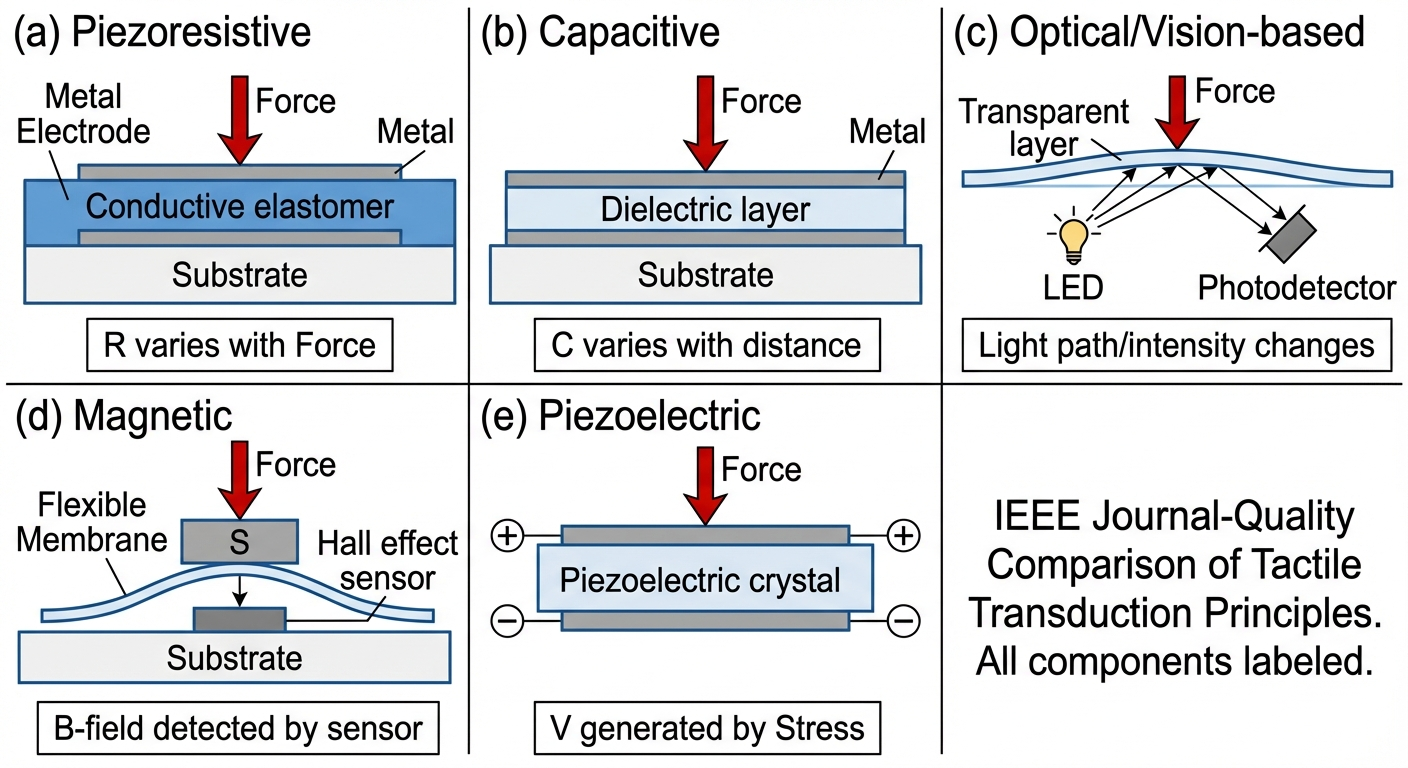
\includegraphics[width=\columnwidth]{../assets/figures/ch02/fig_2_1_transduction_principles_academic.png}
\caption{Taxonomy of tactile transduction principles. Five primary mechanisms---piezoresistive, capacitive, optical/vision-based, magnetic, and piezoelectric---each offer distinct trade-offs in resolution, durability, cost, and form factor.}
\label{fig:transduction_principles}
\end{figure}

\subsection{Transduction Principles}

Tactile sensors convert physical contact into electrical signals via five primary mechanisms, each with distinct trade-offs in resolution, durability, cost, and form factor~\cite{dahiya2010tactile}. Table~\ref{tab:sensors} provides a systematic comparison.

\textbf{Piezoresistive sensors} measure resistance change under pressure. Their simplicity and low cost make them the most widely deployed type. Sundaram et al.~\cite{sundaram2019stag} demonstrated the STAG glove with 548 piezoresistive sensors distributed across the human hand, capturing pressure signatures during natural grasping at high spatial resolution (\emph{Nature}, 2019). The resulting dataset enabled learning grasp-object associations from tactile patterns alone. Key limitations include hysteresis, temperature dependence, and drift under repeated loading, which necessitate periodic recalibration in long-duration applications.

\textbf{Capacitive sensors} detect changes in capacitance between electrode pairs separated by a deformable dielectric. A distinctive advantage is proximity sensing: the ability to detect approaching objects before physical contact occurs, providing pre-contact information unavailable to other sensor types. Murphy et al.~\cite{murphy2025capacitive} deployed 102 capacitive sensors for teaching by demonstration, demonstrating that the combination of pre-contact proximity and post-contact force data enhances policy learning. Susceptibility to electromagnetic interference and wiring complexity remain challenges for dense arrays.

\textbf{Magnetic sensors} combine permanent magnets with Hall-effect or magnetoresistive elements to measure deformation of a soft interface layer. ReSkin~\cite{bhirangi2021reskin} (Meta FAIR/CMU) introduced magnetic elastomer tactile skin at less than \$6 per unit, 2--3~mm thickness, and durability exceeding 50{,}000 interactions. The key innovation is separating the passive sensing surface from the electronics, enabling rapid replacement. AnySkin~\cite{bhirangi2024anyskin} advanced this to achieve \textbf{12-second plug-and-play replacement} without recalibration, maintaining 92\% slip detection accuracy across sensor instances. The OSMO glove~\cite{yin2025osmo} uses 12 three-axis magnetic sensors with MuMetal shielding for simultaneous normal and shear force measurement, serving as a cross-embodiment bridge between human and robot tactile data collection.

\textbf{Piezoelectric sensors} generate charge under dynamic deformation via materials such as PZT or PVDF. They excel at detecting vibration (40--400~Hz) and texture---functionally analogous to Pacinian corpuscles in biological touch~\cite{yu2025texture}. Their dynamic sensitivity makes them ideal for texture classification tasks, though they cannot measure static forces. Energy harvesting potential enables self-powered sensor designs.

\textbf{Optical/vision-based sensors} image the deformation of a transparent gel or elastomer using an embedded camera and reconstruct contact information from the resulting images. This approach has become the dominant paradigm since 2017 and is discussed in detail in the following subsection.

\begin{table*}[t]
\caption{Comparison of Tactile Sensor Technologies}
\label{tab:sensors}
\centering
\begin{tabular}{@{}lccccc@{}}
\toprule
\textbf{Property} & \textbf{Piezoresistive} & \textbf{Capacitive} & \textbf{Optical/Vision} & \textbf{Magnetic} & \textbf{Piezoelectric} \\
\midrule
Spatial resolution & Medium & Medium & Very high & Low--Medium & Low \\
Force range & Wide & Wide & Medium & Medium & Wide (dynamic) \\
Multi-axis sensing & Difficult & Possible & Excellent & Excellent & Difficult \\
Durability & Moderate & Moderate & Low (gel wear) & High & High \\
Cost per unit & Very low & Low & Medium (\$350) & Very low (\$6) & Medium \\
Form factor & Compact & Compact & Bulky (camera) & Compact & Compact \\
Proximity sensing & No & Yes & No & No & No \\
Representative & STAG~\cite{sundaram2019stag} & \cite{murphy2025capacitive} & DIGIT~\cite{lambeta2020digit} & ReSkin~\cite{bhirangi2021reskin} & --- \\
\bottomrule
\end{tabular}
\end{table*}

\begin{figure}[t]
\centering
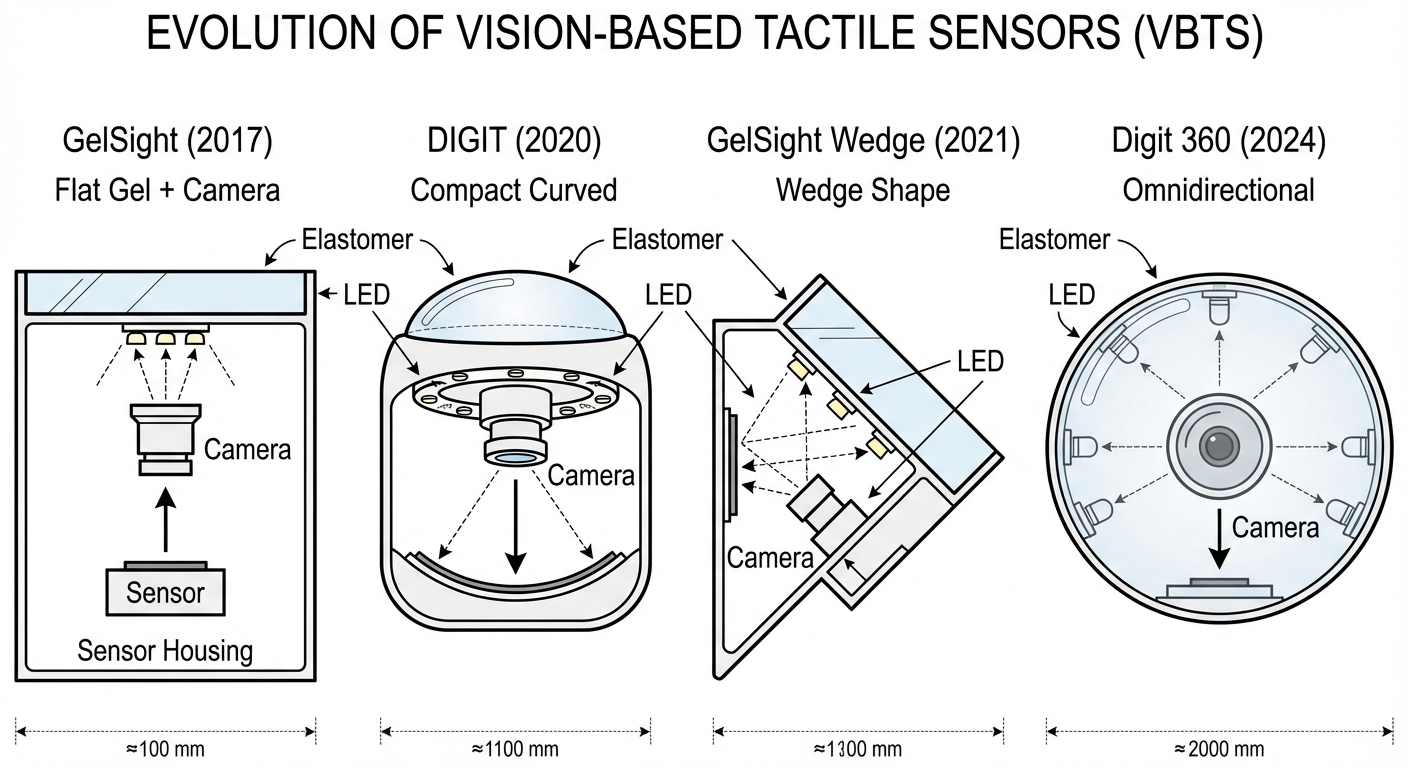
\includegraphics[width=\columnwidth]{../assets/figures/ch02/fig_2_2_vbts_evolution_academic.png}
\caption{Evolution of vision-based tactile sensors (VBTS): from GelSight (2017) through GelSight Wedge and DIGIT to Digit~360, showing progressive improvements in form factor, cost, resolution, and sensing modalities.}
\label{fig:vbts_evolution}
\end{figure}

\subsection{Vision-Based Optical Tactile Sensors}
\label{sec:vbts}

The introduction of GelSight~\cite{yuan2017gelsight} in 2017 marked a paradigm shift in tactile sensing. Using photometric stereo---multiple colored LEDs illuminate a coated elastomeric gel, and a camera captures the resulting shading patterns---GelSight reconstructs 3D contact surface geometry at micrometer resolution. This approach is paradigm-shifting because it imports the entire ecosystem of computer vision tools (CNNs, ViTs, self-supervised learning, diffusion models) to tactile perception, bypassing the need for specialized signal processing pipelines required by electrical transduction methods. With 600+ citations, GelSight established the vision-based tactile sensor (VBTS) family.

\textbf{GelSight Wedge}~\cite{wang2021wedge} (MIT CSAIL, ICRA 2021) redesigned the optical path into a wedge form factor compatible with standard parallel grippers, enabling integration into existing robotic systems rather than requiring custom hardware. This form factor innovation was critical for practical adoption.

\textbf{DIGIT}~\cite{lambeta2020digit} (Meta FAIR, 2020, 400+ citations) achieved the miniaturization and cost reduction needed for widespread adoption. At \$350---over 10$\times$ cheaper than BioTac (\$5K--10K)---and in a compact form factor suitable for mounting on individual fingers of multi-fingered hands, DIGIT became the de facto standard sensor for tactile manipulation research. Its open design catalyzed an ecosystem of downstream work in manipulation, representation learning, and sim-to-real transfer.

\textbf{Digit~360}~\cite{lambeta2024digit360} (Meta FAIR/GelSight, 2024) represents the most comprehensive artificial fingertip to date, integrating approximately 8.3 million taxels, 18+ sensing modalities (3D geometry, normal and shear force, vibration, temperature, proximity), omnidirectional surface coverage, and 1~mN force resolution approaching human sensitivity (3~mN for Meissner corpuscles). Digit~360 integrates multimodal sensing corresponding to multiple human receptor types into a single fingertip, representing the closest attempt yet to a ``complete'' artificial touch organ.

\textbf{Modular design}~\cite{agarwal2025modular} (CMU, \emph{IJRR} 2025) proposed a systematic framework for GelSight-family sensors, enabling customization by modularly combining gel materials, illumination layouts, camera positions, and housings to match application requirements.

The primary limitation of VBTS remains \textbf{durability}. Gel surfaces wear with repeated contact; light sources degrade; dust infiltration and cleaning difficulty constrain long-term industrial operation. When the F-TAC Hand~\cite{zhao2025ftac} placed 17 sensors across the hand, it also introduced 17 potential failure points. AnySkin's 12-second replacement approach~\cite{bhirangi2024anyskin} offers one practical mitigation strategy (see Section~\ref{sec:discussion}).

\subsection{Multi-Axis Sensing}

Normal force alone is insufficient for robust manipulation. Shear (tangential) forces provide critical information for three capabilities: (1)~\textbf{slip detection}---shear force changes are leading indicators of incipient slip, enabling preemptive grip force increase before the object actually slides~\cite{zhao2025slip}; (2)~\textbf{object orientation estimation}---tangential force vectors reveal object tilt relative to the gripper~\cite{hossain2025multiaxis}; and (3)~\textbf{force-noise decoupling}---multi-axis information separates true contact forces from sensor noise and external vibration~\cite{cho2025decoupling}. Multi-dimensional tactile data has also been shown to improve policy sample efficiency in learning-based manipulation.

The OSMO glove~\cite{yin2025osmo} exemplifies practical multi-axis design: 12 three-axis magnetic sensors with MuMetal shielding measure simultaneous normal and shear forces across fingertips and palm. Its open-source design and ``embodiment bridge'' concept---using the same glove on both human and robot to eliminate the tactile domain gap---represent an emerging paradigm for cross-embodiment data collection (see Section~\ref{sec:retarget}).

\subsection{Sensor-Integrated Hand Design}

Sensor technology achieves maximum impact when co-optimized with hand design rather than retrofitted. The F-TAC Hand~\cite{zhao2025ftac} (\emph{Nature Machine Intelligence}, 2025) demonstrated this principle: 17 vision-based tactile sensors were placed based on optimized contact probability distributions, covering 70\% of the hand surface at 0.1~mm resolution. The result was 100\% multi-object grasp success---a direct demonstration that integrated tactile feedback transforms manipulation performance. 3D-ViTac~\cite{huang2024vitac} (CoRL 2024) fused dense tactile sensors (3~mm$^2$ resolution) with vision into a unified 3D representation, achieving 85--90\% success on bimanual dexterous tasks versus 45--50\% with vision only.

\subsection{Emerging Directions}

\textbf{Neuromorphic tactile sensors} mimic the biological nervous system's event-driven processing to maximize energy efficiency and temporal resolution. NRE-skin~\cite{gao2025nreskin} (\emph{PNAS}, 2025) implements a hierarchical neural-inspired architecture enabling high-resolution touch sensing, active pain/injury detection with local reflexes, and modular quick-release repair. Spike-based encoding achieves 10$\times$ super-resolution through CMOS/memristor hardware combined with spiking neural network (SNN) decoding~\cite{various2025spike}. Bioinspired spiking architectures have demonstrated efficient tactile encoding under energy constraints (\emph{Nature Communications}, 2026).

\textbf{Self-healing electronic skin} addresses durability through materials science. Multisensory e-skin with decoupled pressure-temperature sensing and self-healing properties~\cite{various2025eskin} has the potential to fundamentally resolve the sensor durability challenge in industrial environments.

\textbf{Physically-based rendering (PBR) for sensor design}~\cite{various2025pbr} (\emph{Nature Communications Engineering}, 2025) enables simulation-driven design of optical tactile sensors, reducing fabrication trial-and-error and supporting digital twin-based development workflows.
